%%%%%%%%%%%%%%%%%%%%%%%%%%%%%%%%%%%%%%%%%
% The Legrand Orange Book
% LaTeX Template
% Version 3.1 (February 18, 2022)
% Compiling this template:
% This template uses biber for its bibliography and makeindex for its index.
% When you first open the template, compile it from the command line with the 
% commands below to make sure your LaTeX distribution is configured correctly:
%
% 1) pdflatex mainv2
% 2) makeindex mainv2.idx -s indexstyle.ist
% 3) biber mainv2
% 4) pdflatex mainv2 x 2


%Atención
%Está prohibido usar simbolos en \index{•}
% After this, when you wish to update the bibliography/index use the appropriate
% command above and make sure to compile with pdflatex several times 
% afterwards to propagate your changes to the document.
%
%%%%%%%%%%%%%%%%%%%%%%%%%%%%%%%%%%%%%%%%%

%----------------------------------------------------------------------------------------
%	PACKAGES AND OTHER DOCUMENT CONFIGURATIONS
%----------------------------------------------------------------------------------------

\documentclass[
	12pt, % Default font size, select one of 10pt, 11pt or 12pt
	fleqn, % Left align equations
	a4paper, % Paper size, use either 'a4paper' for A4 size or 'letterpaper' for US letter size
	oneside, % Uncomment for oneside mode, this doesn't start new chapters and parts on odd pages (adding an empty page if required), this mode is more suitable if the book is to be read on a screen instead of printed
]{LegrandOrangeBook}

% Book information for PDF metadata, remove/comment this block if not required 
\hypersetup{
	pdftitle={Pasos por Telecomunicaciones II}, % Title field
	pdfauthor={Jose Hancco}, % Author field
	pdfsubject={Educación}, % Subject field
	pdfkeywords={Telecomunicaciones, UNSA, Pregrado, Señales}, % Keywords
	pdfcreator={LaTeX}, % Content creator field
}

\addbibresource{sample.bib} % Bibliography file

\definecolor{ocre}{RGB}{63, 76, 83} % Define the color used for highlighting throughout the book, replace it with average color for a better presentation:
% Background.pdf -> Average color=63,76,83
% Background1.pdf -> Average color=31,31,40
% Background2.pdf -> Average color=123,119,101
% Background3.pdf -> Average color=103,61,76
\chapterimage{Final1.jpg} % Chapter heading image
\chapterspaceabove{6.5cm} % Default whitespace from the top of the page to the chapter title on chapter pages
\chapterspacebelow{6.75cm} % Default amount of vertical whitespace from the top margin to the start of the text on chapter pages

%----------------------------------------------------------------------------------------

\begin{document}

%----------------------------------------------------------------------------------------
%	TITLE PAGE
%----------------------------------------------------------------------------------------

\begingroup
\thispagestyle{empty} % Suppress headers and footers on the title page
\begin{tikzpicture}[remember picture,overlay]
\node[inner sep=0pt] (background) at (current page.center) {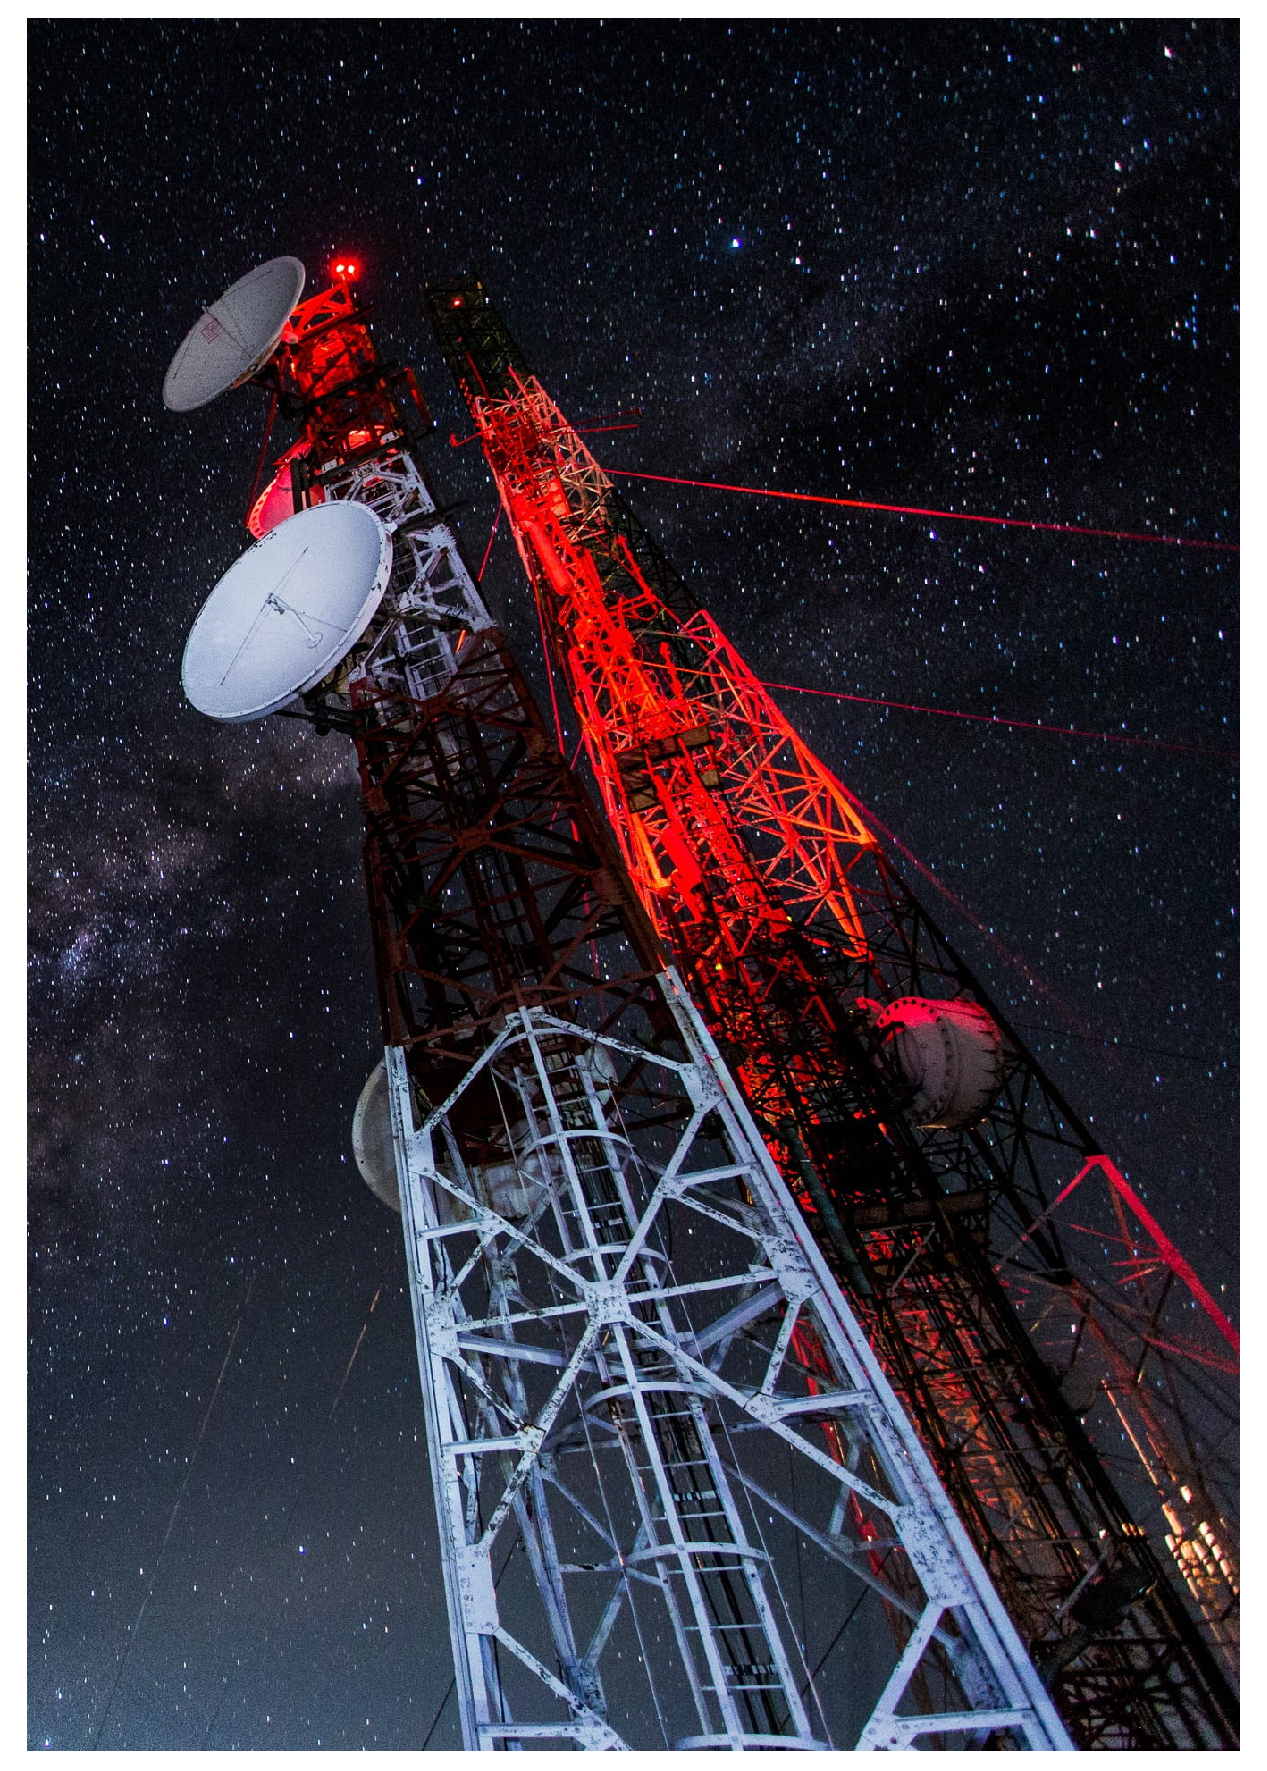
\includegraphics[width=\paperwidth]{background1.pdf}};%here you change your bookcover background
\draw (current page.center) node [fill=ocre!30!white,fill opacity=0.6,text opacity=1,inner sep=1cm]{\Huge\centering\bfseries\sffamily\parbox[c][][t]{\paperwidth}{\centering Pasos por Telecomunicaciones II\\[15pt] % Book title
{\Large Notas de un estudiante}\\[20pt] % Subtitle
{\huge Jose Antonio Hancco M.}}}; % Author name
\end{tikzpicture}
\vfill
\endgroup

%----------------------------------------------------------------------------------------
%	COPYRIGHT PAGE
%----------------------------------------------------------------------------------------

\newpage
~\vfill
\thispagestyle{empty}

\noindent Copyright \copyright\ 2022 Jose Hancco\\ % Copyright notice

\noindent \textsc{Libro libre de usos}\\ % Publisher

\noindent \textsc{https://github.com/Yasperterian}\\ % URL

\noindent Con licencia de Creative Commons Attribution-NonCommercial 3.0 Unported License (la ``Licencia''). No puede usar este archivo excepto de conformidad con la Licencia. Puede obtener una copia de la Licencia en \url{http://creativecommons.org/licenses/by-nc/3.0}. A menos que lo exija la ley aplicable o se acuerde por escrito, el software distribuido bajo la Licencia se distribuye \textsc{``tal cual'', sin garantías ni condiciones de ningún tipo}, ya sea expresa o implícita. Consulte la Licencia para conocer el idioma específico que rige los permisos y las limitaciones en virtud de la Licencia.\\ % License information, replace this with your own license (if any)

\noindent \textit{Primera edición, septiembre 2022} % Printing/edition date

\noindent Si existe algún error, crees que una sección se puede mejorar o dar cualquier tipo de \textit{feedback} acerca del libro no dudes y mándame un correo a \textit{jhanccoma@unsa.edu.pe}, te responderé lo más pronto que pueda y gracias por mejorar este libro de todos y para todos.
%----------------------------------------------------------------------------------------
%Dedicate
%----------------------------------------------------------------------------------------
\clearpage
\begin{center}
    \thispagestyle{empty}
    \vspace*{\fill}
    \textit{Dedicatoria aquí}
    \vspace*{\fill}
\end{center}
\clearpage
%----------------------------------------------------------------------------------------
%	TABLE OF CONTENTS
%----------------------------------------------------------------------------------------

%\usechapterimagefalse % If you don't want to include a chapter image, use this to toggle images off - it can be enabled later with \usechapterimagetrue

\chapterimage{chapter_head_generalindex3.pdf} % Table of contents heading image

\pagestyle{empty} % Disable headers and footers for the following pages

\tableofcontents % Print the table of contents itself

\cleardoublepage % Forces the first chapter to start on an odd page so it's on the right side of the book

\pagestyle{fancy} % Enable headers and footers again
%----------------------------------------------------------------------------------------
%	PART
%----------------------------------------------------------------------------------------
\section*{Libros recomendados:}
\begin{itemize}
\item Fundamentos de circuitos eléctricos\cite{alexander2013fundamentos}
\item Signals and Systems Using MATLAB\cite{chaparro2018signals}
\item Procesamiento de señales analógicas y digitales\cite{ambardar1995analog}
\item Física Para Ciencias E Ingeniería. Vol 1\cite{serway2018fisica1}
\item Física Para Ciencias E Ingeniería. Vol 2\cite{serway2018fisica2}
\item Cálculo de una variable: trascendentes tempranas. 7ma edición \cite{stewart12calculo}
\item Análisis de Fourier\cite{hsu1998analisis}
\item Matemáticas Avanzadas Para Ingeniería\cite{o2014matematicas}
\item Métodos numéricos para ingenieros\cite{chapra2013metodos}
\item Comunicaciones y redes de computadores\cite{stallings2004comunicaciones}
\item Electrónica: teoría de circuitos y dispositivos electrónicos\cite{boylestad1989electronica}
\item Fundamentos de sistemas digitales\cite{floyd2006fundamentos}
\item Tratamiento de señales en tiempo discreto\cite{oppenheim2011tratamiento}
\item Tratamiento digital de señales\cite{proakis2007tratamiento}
\item Sistemas de comunicación digitales y análogos\cite{couchsistemas}
\item Data communication and networking\cite{forouzan2007data}
\item Life Pre-Intermediate 2e\cite{hughes2017life}
\item Redes de computadoras\cite{tanenbaum2012computer}
\item Líneas de transmisión\cite{velalineas1999}
\end{itemize}
%----------------------------------------------------------------------------------------
%	NEW CHAPTER
%----------------------------------------------------------------------------------------
\part{Samples}
\chapterimage{chapter_head_T2.pdf} % Chapter heading image

\chapter{Unidad I}

\section{Theorems}\index{Theorems}

This is an example of theorems.

\subsection{Several equations}\index{Theorems!Several Equations}
This is a theorem consisting of several equations.

\begin{theorem}[Name of the theorem]
In $E=\mathbb{R}^n$ all norms are equivalent. It has the properties:
\begin{align}
& \big| ||\mathbf{x}|| - ||\mathbf{y}|| \big|\leq || \mathbf{x}- \mathbf{y}||\\
&  ||\sum_{i=1}^n\mathbf{x}_i||\leq \sum_{i=1}^n||\mathbf{x}_i||\quad\text{where $n$ is a finite integer}
\end{align}
\end{theorem}

\subsection{Single Line}\index{Theorems!Single Line}
This is a theorem consisting of just one line.

\begin{theorem}
A set $\mathcal{D}(G)$ in dense in $L^2(G)$, $|\cdot|_0$. 
\end{theorem}

%------------------------------------------------

\section{Definitions}\index{Definitions}

This is an example of a definition. A definition could be mathematical or it could define a concept.

\begin{definition}[Definition name]
Given a vector space $E$, a norm on $E$ is an application, denoted $||\cdot||$, $E$ in $\mathbb{R}^+=[0,+\infty[$ such that:
\begin{align}
& ||\mathbf{x}||=0\ \Rightarrow\ \mathbf{x}=\mathbf{0}\\
& ||\lambda \mathbf{x}||=|\lambda|\cdot ||\mathbf{x}||\\
& ||\mathbf{x}+\mathbf{y}||\leq ||\mathbf{x}||+||\mathbf{y}||
\end{align}
\end{definition}

%------------------------------------------------

\section{Notations}\index{Notations}

\begin{notation}
Given an open subset $G$ of $\mathbb{R}^n$, the set of functions $\varphi$ are:
\begin{enumerate}
\item Bounded support $G$;
\item Infinitely differentiable;
\end{enumerate}
a vector space is denoted by $\mathcal{D}(G)$. 
\end{notation}

%------------------------------------------------

\section{Remarks}\index{Remarks}

This is an example of a remark.

\begin{remark}
The concepts presented here are now in conventional employment in mathematics. Vector spaces are taken over the field $\mathbb{K}=\mathbb{R}$, however, established properties are easily extended to $\mathbb{K}=\mathbb{C}$.
\end{remark}

%------------------------------------------------

\section{Corollaries}\index{Corollaries}

This is an example of a corollary.

\begin{corollary}[Corollary name]
The concepts presented here are now in conventional employment in mathematics. Vector spaces are taken over the field $\mathbb{K}=\mathbb{R}$, however, established properties are easily extended to $\mathbb{K}=\mathbb{C}$.
\end{corollary}

%------------------------------------------------

\section{Propositions}\index{Propositions}

This is an example of propositions.

\subsection{Several equations}\index{Propositions!Several Equations}

\begin{proposition}[Proposition name]
It has the properties:
\begin{align}
& \big| ||\mathbf{x}|| - ||\mathbf{y}|| \big|\leq || \mathbf{x}- \mathbf{y}||\\
&  ||\sum_{i=1}^n\mathbf{x}_i||\leq \sum_{i=1}^n||\mathbf{x}_i||\quad\text{where $n$ is a finite integer}
\end{align}
\end{proposition}

\subsection{Single Line}\index{Propositions!Single Line}

\begin{proposition} 
Let $f,g\in L^2(G)$; if $\forall \varphi\in\mathcal{D}(G)$, $(f,\varphi)_0=(g,\varphi)_0$ then $f = g$. 
\end{proposition}

%------------------------------------------------

\section{Examples}\index{Examples}

This is an example of examples.

\subsection{Equation and Text}\index{Examples!Equation and Text}

\begin{example}
Let $G=\{x\in\mathbb{R}^2:|x|<3\}$ and denoted by: $x^0=(1,1)$; consider the function:
\begin{equation}
f(x)=\left\{\begin{aligned} & \mathrm{e}^{|x|} & & \text{si $|x-x^0|\leq 1/2$}\\
& 0 & & \text{si $|x-x^0|> 1/2$}\end{aligned}\right.
\end{equation}
\end{example}

\subsection{Paragraph of Text}\index{Examples!Paragraph of Text}

\begin{example}[Example name]
\lipsum[2]
\end{example}

%------------------------------------------------

\section{Exercises}\index{Exercises}

This is an example of an exercise.

\begin{example}
This is a good place to ask a question to test learning progress or further cement ideas into students' minds.
\end{example}

%------------------------------------------------

\section{Problems}\index{Problems}

\begin{problem}
What is the average airspeed velocity of an unladen swallow?
\end{problem}

%------------------------------------------------

\section{Vocabulary}\index{Vocabulary}


\begin{vocabulary}[Word]
Definition of word.
\end{vocabulary}

\section{Table}\index{Table}

\begin{table}[h]
\centering
\begin{tabular}{l l l}
\toprule
\textbf{Treatments} & \textbf{Response 1} & \textbf{Response 2}\\
\midrule
Treatment 1 & 0.0003262 & 0.562 \\
Treatment 2 & 0.0015681 & 0.910 \\
Treatment 3 & 0.0009271 & 0.296 \\
\bottomrule
\end{tabular}
\caption{Table caption}
\label{tab:example} % Unique label used for referencing the table in-text
%\addcontentsline{toc}{table}{Table \ref{tab:example}} % Uncomment to add the table to the table of contents
\end{table}

Referencing Table \ref{tab:example} in-text automatically.

%------------------------------------------------

\section{Figure}\index{Figure}
\begin{figure}[h]
\centering
\includegraphics[scale=0.5]{placeholder.jpg}
\caption{Figure caption}
\label{fig:placeholder} % Unique label used for referencing the figure in-text
%\addcontentsline{toc}{figure}{Figure \ref{fig:placeholder}} % Uncomment to add the figure to the table of contents
\end{figure}

Referencing Figure \ref{fig:placeholder} in-text automatically.

%----------------------------------------------------------------------------------------
%	NEW CHAPTER
%----------------------------------------------------------------------------------------
\part{Antenas}
\chapterimage{chapter_head_ANT.pdf} % Chapter heading image

\chapter{Unidad I}
\section{Introducción}
Como siempre, antes de este curso hay que recordar algunos términos o conceptos para poder entender cosas que se vienen. Empezamos con las unidades logarítmicas:
\begin{align*}
Belio&=\log\left(\frac{P_{out}}{P_{in}}\right)\\
Decibelio(dB)&=10\cdot\log\left(\frac{P_{out}}{P_{in}}\right)\\
Decibelio(dB)&=20\cdot\log\left(\frac{V_{out}}{V_{in}}\right)\\
Neper(Np)&=ln\left(\frac{V_{out}}{V_{in}}\right)
\end{align*}
Asimismo debemos tener en cuenta las demás medidads respecto a un valor como 1mW, 1W, 1V, etc.\footnote{Estas puedes ser vistas en la sección \textbf{Decibelios} en el capítulo de \textbf{Ingeniería en mantenimiento}.}
Otros conceptos importantes a recordar son:
\begin{definition}[Longitud de Onda]
\begin{equation}
\lambda=\frac{v}{f}
\end{equation}
Donde:
\begin{itemize}
\item $\lambda$: Longitud de onda. (m)
\item \textbf{v}: Velocidad, si el medio es el aire o espacio libre: v=c=300000 km/s=300000000 m/s (m/s)
\item $f$: Frecuencia. (Hz)
\end{itemize}
\end{definition}
\begin{definition}[Temperatura]
\begin{equation}
\frac{°C}{5}=\frac{°F-32}{9}=\frac{K-273}{5}=\frac{R-492}{9}
\end{equation}
Despejando podemos obtener:
\begin{align*}
°C=\frac{5}{9}\left(°F-32\right)\\
K=°C+273\\
R=°F+460
\end{align*}
\end{definition}
Además debemos recordar las bandas y frecuencias designadas por la ITU:
\begin{table}[H]
\centering
\begin{tabular}{|c|c|c|c|}
\hline
\rowcolor[HTML]{9698ED} 
N° de banda & Rango de frecuencia & Indicativo & Propagación                    \\ \hline
2           & 30-300 Hz           & ELF        & Onda terrestre                 \\ \hline
3           & 0.3-3 KHz           & SLF        & Onda terrestre                 \\ \hline
4           & 3-30 KHz            & VLF        & Onda terrestre                 \\ \hline
5           & 30-300 KHz          & LF         & Onda terrestre y superficial   \\ \hline
6           & 0.3-3 MHz           & MF         & Onda superficial               \\ \hline
7           & 3-30 MHz            & HF         & Onda superficial y Ionosférica \\ \hline
8           & 30-300 MHz          & VHF        & Onda Ionosférica y directa     \\ \hline
9           & 0.3-3 GHz           & UHF        & Onda directa                   \\ \hline
10          & 3-30 GHz            & SHF        & Onda directa                   \\ \hline
11          & 30-300 GHz          & EHF        & Onda directa e infrarojo       \\ \hline
12          & 0.3-3 THz           &            & Luz infraroja                  \\ \hline
13          & 3-30 THz            &            & Luz infraroja                  \\ \hline
14          & 30-300 THz          &            & Luz infraroja                  \\ \hline
15          & 0.3-3 PHz           &            & Luz visible                    \\ \hline
16          & 3-30 PHz            &            & Luz ultravioleta               \\ \hline
17          & 30-300 PHz          &            & Rayos X                        \\ \hline
18          & 0.3-3 EHz           &            & Rayos X                        \\ \hline
19          & 3-30 EHz            &            & Rayos cósmicos                 \\ \hline
\end{tabular}
\caption{Designación de bandas CCIR por la ITU.}
\end{table}
Los medios de transmisión:
\begin{table}[H]
\resizebox{\textwidth}{!}{
\begin{tabular}{|c|c|c|c|}
\hline
\rowcolor[HTML]{9698ED} 
Medio de transmisión                                                                         & Banda de frecuencia & Longitud de onda & Aplicación principal                                                                                                                                         \\ \hline
\begin{tabular}[c]{@{}c@{}}Par de alambres,\\ cable multipar\end{tabular}                    & 30-300 Hz           & 10000-1000 Km    & Comunicación submarina                                                                                                                                       \\ \hline
\begin{tabular}[c]{@{}c@{}}Par de alambres,\\ cable multipar\end{tabular}                    & 0.3-3 KHz           & 1000-100 Km      & \begin{tabular}[c]{@{}c@{}}Telefonía, transmisión de datos,\\ telex, fax.\end{tabular}                                                                       \\ \hline
\begin{tabular}[c]{@{}c@{}}Par de alambres,\\ cable multipar,\\ ondas de tierra\end{tabular} & 3-30 KHz            & 100-10 Km        & \begin{tabular}[c]{@{}c@{}}Telefonía de onda portadora baja,\\ capacidad, navegación y radiotelegrafía.\end{tabular}                                         \\ \hline
\begin{tabular}[c]{@{}c@{}}Par de alambres,\\ ondas de tierra\end{tabular}                   & 30-300 KHz          & 10-1 Km          & \begin{tabular}[c]{@{}c@{}}Telefonía de onda portadora mediana\\ capacidad, radiofaro, navegación,\\ radiodifusión onda larga.\end{tabular}                  \\ \hline
\begin{tabular}[c]{@{}c@{}}Cable coaxial, ondas\\ de cielo\end{tabular}                      & 0.3-3 MHz           & 1000-100 m       & \begin{tabular}[c]{@{}c@{}}Radiodifusión, AM, radio aficionados,\\ radio móvil.\end{tabular}                                                                 \\ \hline
\begin{tabular}[c]{@{}c@{}}Cable coaxial, cable UTP cat 3-4,\\ ondas de cielo\end{tabular}   & 3-30 MHz            & 100-10m          & \begin{tabular}[c]{@{}c@{}}Radio aficionados, comunicaciones milirares,\\ marítimas, radio telefonía movil.\end{tabular}                                     \\ \hline
\begin{tabular}[c]{@{}c@{}}Cable coaxial, cable UTP cat 5,\\ ondas directas\end{tabular}     & 30-300 MHz          & 10-1 m           & \begin{tabular}[c]{@{}c@{}}TV, radiodifusión FM, multiacceso radial,\\ radio enlaces, direccionales.\end{tabular}                                            \\ \hline
Ondas directas                                                                               & 0.3-3 GHz           & 100-10 cm        & \begin{tabular}[c]{@{}c@{}}TV, telemetría por radar, comunicaiones\\ militares por satélite, telefonía celular, radio\\ de espectro ensanchado.\end{tabular} \\ \hline
Guía de onda, línea visual                                                                   & 3-30 GHz            & 10-1 cm          & \begin{tabular}[c]{@{}c@{}}Comunicaiones vía satélite, radio enlace\\ direccional analógico y digítal, operación\\ aérea por radar.\end{tabular}             \\ \hline
Guía de onda, línea visual.                                                                  & 30-300 GHz          & 1-0.1 cm         & \begin{tabular}[c]{@{}c@{}}Comunicación militar por satelite, \\ radio astronomia, aterrizaje por radar.\end{tabular}                                        \\ \hline
Fibra óptica                                                                                 & 100-1000 THz        & 3-0.3 pm         & \begin{tabular}[c]{@{}c@{}}Telefonia muy alta capacidad, servicios de\\ banda ancha (SONET, SDH y ATM),\\ video conferencia, CATV por F.O.\end{tabular}      \\ \hline
\end{tabular}
}
\end{table}
\subsection{Ancho de banda y capacidad de información}\index{Ancho de banda y capacidad de información}
Las limitaciones más importantes para el funcionamiento de una sistema de comunicaciones son el \textbf{ruido} y el \textbf{ancho de banda}. El ancho de banda de un canal de comunicación es la diferencia entre la frecuencia máxima y mínima que puede pasar por el canal. El ancho de banda de un canal de comunicación debe ser igual o mayor que el ancho de banda de la información.
\begin{definition}[Ley de Hartley]
Es la medida de cuanta información se puede transferir a través de un sistema de comunicaciones en un determinado tiempo.
\begin{equation}
I\approx B\times t
\label{eq:hartley}
\end{equation}
Donde:
\begin{itemize}
\item \textbf{I}: Capacidad de información.
\item \textbf{B}: Ancho de banda. (Hz)
\item \textbf{t}: Tiempo de transmisión. (s)
\end{itemize}
\end{definition}
\begin{notation}
Se requieren \textbf{3 KHz} de ancho de banda para transmitir las señales telefónicas con calidad de voz.\\
Se asignas 200 KHz para transmisión comercial de FM para música, con alta fidelidad.\\
Se requieren casi 6 MHz de ancho de banda para emitir señales de televisión de alta calidad
\end{notation}
Otra medida que debemos saber es:
\begin{definition}[Capacidad de información de un canal digital]
Shannon relacionó la capacidad de información de un canal de comunicaciones, en bits por segundo (bps), con el ancho de banda y la relación señal a ruido: 
\begin{equation}
I=B\cdot\log_2(1+S/N)
\label{eq:shannon}
\end{equation}
Donde:
\begin{itemize}
\item I: Capacidad de información. (bps)
\item B: Ancho de banda. (Hz)
\item S/N: Relación señal a ruido.
\end{itemize}
\end{definition}
\subsection{Ruido}\index{Ruido}
Energía eléctrica no deseable presente en la banda útil del circuito de comunicación. Se puede clasificar el ruido en dos categorías:
\begin{enumerate}
\item \textbf{Correlacionado}: Solo existe cuando hay una señal. Es aquel que se relaciona mutuamente con la señal, y no puede estar en un circuito a menos que haya una señal de entrada.
Se produce por amplificación no lineal, e incluye la distorsión armónica (cuando se producen las armónicas no deseadas de una señal, debido a una amplificación no lineal) y de intermodulación (generación de frecuencias indeseables de suma o diferencia), ya que las dos son formas de distorsión no lineal.

\item \textbf{No Correlacionado}: Está presente siempre, haya o no señal. El ruido No Correlacionado puede sub dividirse en dos categorías generales:
\begin{enumerate}
\item \textbf{El Ruido Externo }es el que se genera fuera del dispositivo o circuito. Hay tres causas principales de ruido Externo:
\begin{enumerate}
\item \textbf{Ruido atmosférico}: Perturbaciones eléctricas naturales. Electricidad estática (rayos)
\item \textbf{Ruido extraterrestre}: Señales eléctricas originadas fuera de la atmósfera terrestre (solar y cósmico)
\item \textbf{Ruido hecho por el hombre}: Su puente principal son mecanismos que producen chispas, ruido industrial (conmutadores, generadores, lámparas fluorescentes)
\end{enumerate}
\item \textbf{El Ruido Interno} es la interferencia eléctrica generada dentro de un dispositivo o circuito. Las causas principales son:
\begin{enumerate}
\item \textbf{Ruido Térmico}: Asociado con el movimiento rápido y aleatorio de electrones libre, producido por la agitación térmica.
\item \textbf{Ruido de Tiempo de Tránsito}: Variación irregular y aleatoria, producida por la modificación de una corriente de portadores, cuando pasa de la entrada a la salida de un dispositivo.
\item \textbf{Ruido de Disparo}: Se debe a la llegada aleatoria de portadoras al elemento de salida de un dispositivo electrónico (diodo, FET, transistor bipolar).
\end{enumerate}
\end{enumerate}
\end{enumerate}
\subsection{Ruido térmico}\index{Ruido térmico}
Es el movimiento aleatorio de los electrones libres dentro de un conductor, causado por la agitación térmica.
Llamado también: Movimiento Browniano por su descubridor Robert Brown, Ruido de Johnson en honor a quien lo relacionó con el movimiento de los electrones y Ruido Blanco porque se produce en todas las frecuencias.
\begin{definition}[Potencia de ruido térmico]
\begin{equation}
P_{tn}=K\cdot T\cdot B
\label{eq:ruido termico}
\end{equation}
Donde:
\begin{itemize}
\item $P_{tn}$: Potencia del ruido. (W) térmico\footnote{tn:thermal noise o ruido térmico.} (W)
\item \textbf{K:} Constante de Boltzmann= $1.38\times\basedec{-23} J/°K$.
\item \textbf{T}: Temperatura absoluta. (°K)
\item \textbf{B}: Ancho de banda. (Hz)
\end{itemize}
Alternativamente, el ruido térmico puede ser expresado en dBm, para ello debemos usar la siguiente expresión:
\begin{equation}
P_{tn}(dBm)=10\cdot\log\left(\frac{K\cdot T\cdot B}{0.001}\right)
\label{eq:ruido termico log}
\end{equation}
En temperatura ambiente, el ruido térmico ambiente:
\begin{equation}
P_{tn}(dBm)=-174 dBm+10\log(B)
\label{eq:ruido termico ambiente}
\end{equation}
\end{definition}
\begin{definition}[Voltaje ruido térmico]
\begin{equation}
V_{tn}=\sqrt{4\cdot R\cdot K\cdot T\cdot B}
\label{eq:voltaje ruido termico}
\end{equation}
Donde:
\begin{itemize}
\item \textbf{R}: Resistencia interna. ($\Omega$)
\item \textbf{$V_{tn}$}: Voltaje RMS del ruido. (V)
\end{itemize}
\end{definition}
\begin{notation}
Para la máxima potencia transferencia de potencia $R_L=R_I$.
\end{notation}
\begin{definition}[Relación señal a ruido-SNR]
Es la relación en decibelios entre la potencia de la señal(S) y la potencia del ruido(N):
\begin{equation}
\label{eq:snr}
SNR=10\log_{10}\left(\frac{S}{N}\right)=20\log_{10}\left(\frac{V_s}{V_n}\right)
\end{equation}
\end{definition}
\begin{remark}
El \textbf{factor a ruido} se define como el cociente entre la potencia SNR de entrada y potencia SNR de salida. Por consecuencia, la \textbf{cifra de ruido} es el factor de ruido expresado en dB.
\end{remark}
\begin{notation}
Para voltaje, 6dB indica que la salida es dos veces el valor de la entrada, es decir: Si la entrada es 1, la salida será 2. Para potencia, 3dB indica lo mismo: el valor de la salida es dos veces el valor de la entrada.
\end{notation}
\subsection{Ángulo crítico}\index{Ángulo crítico}
Debemos recordar ecuaciones como Ley de Snell,
\begin{definition}[Ley de Snell]
\begin{align}
n_1\sin\theta_1&=n_2\sin\theta_2\\
\sqrt{\epsilon_1}\sin\theta_1&=\sqrt{\epsilon_2}\sin\theta_2
\label{eq:snell}
\end{align}
Donde:
\begin{itemize}
\item $n$: Indice de refracción.
\item $\theta$ Ángulo de refracción.
\item $\epsilon$: Permitividad relativa del material.
\end{itemize}
\end{definition}
\begin{figure}[H]
\centering
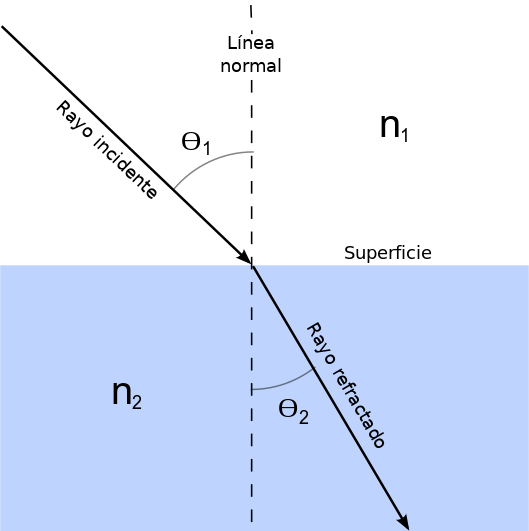
\includegraphics[width=0.6\linewidth]{Ant/Ant6.png}
\caption{Ley de Snell}
\end{figure}
dentro de ella una que usaremos es la del \textit{ángulo crítico}:
\begin{center}
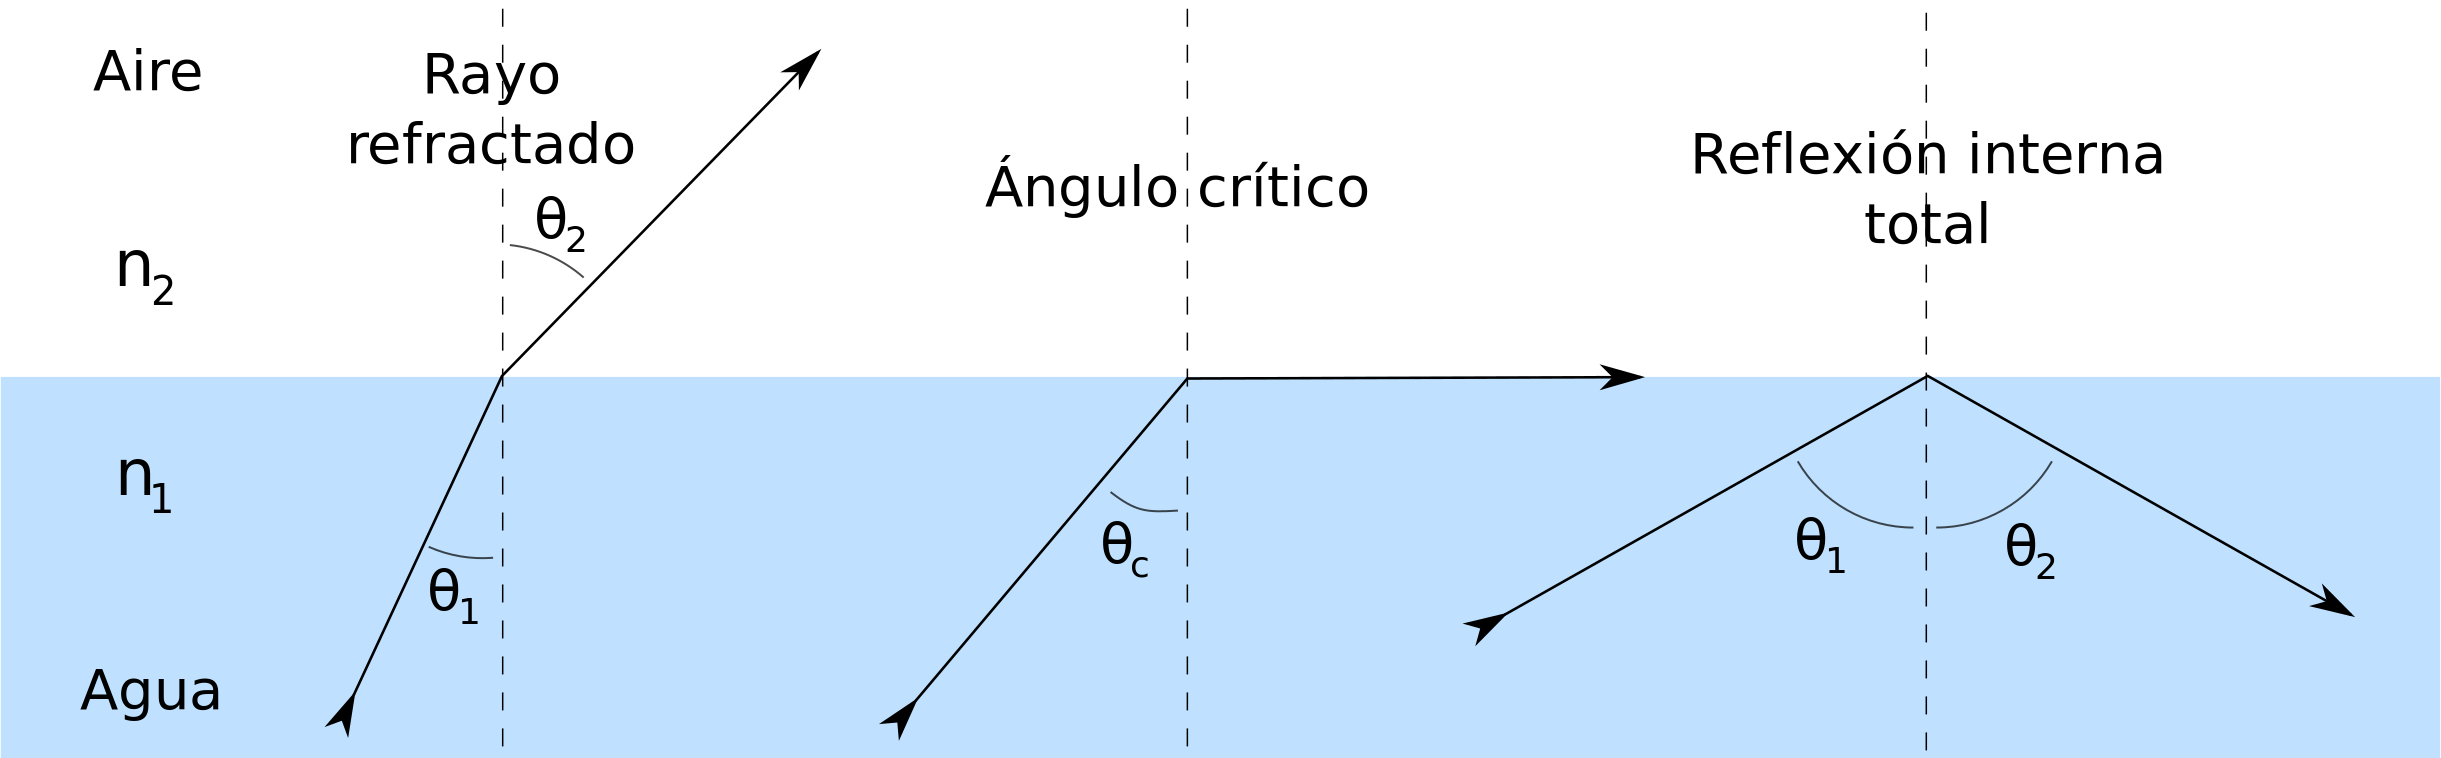
\includegraphics[width=0.8\linewidth]{Ant/Ant1.png}
\end{center}
La forma de obtener el ángulo crítico es:
\begin{equation}
\sin\theta_c=\frac{n_2}{n_1}
\label{eq: angulo critico}
\end{equation}
\begin{notation}
El índice de refracción esta definido como el cociente de la \textbf{velocidad de la luz en el vacío} entre la \textbf{velocidad de la luz del medio donde se propaga}. Generalmente se utiliza la velocidad de la luz en el vacío (\textit{c}) como medio de referencia para cualquier materia, aunque durante la historia se han utilizado otras referencias, como la velocidad de la luz en el aire. En el caso de la luz, es igual a $n=\sqrt{\epsilon_r\cdot\mu_r}$. Para la mayoría de los materiales, la \textbf{permeabilidad magnética relativa} ($\mu_r$) es muy cercano a 1 en frecuencias ópticas, es decir, luz visible, por lo tanto, \textit{n} es aproximadamente $\sqrt{\epsilon_r}$
\end{notation}
\subsection{Repaso: Propagación de ondas electromagnéticas}
La propagación de OEM por el espacio libre se suele llamar propagación de radiofrecuencia o radio propagación. Las OEM, en el espacio libre se propagan en línea recta a la velocidad de la luz ($3\basedec{8}m/s$). 
\begin{definition}[Distancia máxima de línea]
\begin{subequations}
\begin{align}
d_{max}&=\sqrt{2\cdot h}
\label{eq:dist millas} \\
d_{max}&=\sqrt{17\cdot h})\label{eq:dist km}
\end{align}
\end{subequations}
Donde:
\begin{itemize}
\item $d_{max}$: Distancia máxima de línea de vista. (millas ó Km)
\item \textbf{h}: Altura (Pies ó m)\footnote{La distancia será en millas si se trabaja con la ecuación \ref{eq:dist millas}, donde la altura debe ser introducida en pies. Para la ecuación \ref{eq:dist km}, la distancia estará en metros y la altura en metros.}
\end{itemize}
\end{definition}
Hablemos también de las \textbf{pérdidas por trayectoria}. El modelo de pérdida por trayectoria en el espacio libre es usado para predecir la intensidad del nivel de recepción cuando el transmisor y receptor tienen una trayectoria de línea de vista clara, sin obstrucciones entre ellos.
\begin{definition}[Pérdidas por trayectoria]
\begin{subequations}
\begin{align}
L_p=\left(\frac{4\pi\cdot d}{\lambda}\right)^2=\left(\frac{4\pi\cdot d\cdot f}{c}\right)^2
\label{eq:perdidas trayec adimensional} \\
L_p=20\cdot\log\left(\frac{4\pi\cdot d\cdot f}{c}\right)=20\cdot\log\left(\frac{4\pi}{c}\right)+20\cdot\log(f)+20\cdot\log(d)\label{eq:perdidas trayec db}
\end{align}
\end{subequations}
Donde:
\begin{itemize}
\item \textbf{d}: Distancia. (m)
\item \textbf{\textit{f}}: Frecuencia. (Hz)
\item \textbf{\textit{c}}: Velocidad de la luz.
\item $\lambda$: Longitud de onda. (m)
\end{itemize}
Si la distancia se expresa en Km y la frecuencia en MHz:
\begin{equation}
L_p(dB)=32.4+20\cdot\log(f)+20\log(d)
\end{equation}
\end{definition}
Otro término usado es la \textbf{polarización}, recordando que una OEM contiene un campo eléctrico y un campo magnético que forman 90° entre sí. Por lo tanto, la polarización de una OEM plana, no es mas que la orientación dle vector campo eléctrico respecto a la superficie de la tierra.\\
\textbf{Tipos de polarización:}
\begin{enumerate}
\item \textbf{Polarización lineal}: Si la polarización permanece constante. Las formas lineales son:(Fig. \ref{fig:pol lin})
\begin{enumerate}
\item \textbf{Polarización Horizontal}: Campo eléctrico paralelo a la superficie de la tierra.
\item \textbf{Polarización Vertical}: Campo eléctrico perpendicular a la superficie terrestre.
\end{enumerate}
\item \textbf{Polarización Circular}: Luz polarizada circularmente consta de dos ondas electromagnéticas planas perpendiculares con una diferencia de fase de 90º. (Fig. \ref{fig:pol circ})
\item \textbf{Polarización elíptica}: La luz polarizada elípticamente consiste de dos ondas perpendiculares de amplitudes desiguales y con una diferencia de fase de 90º. (Fig. \ref{fig:pol elip})
\end{enumerate}
\begin{figure}[]
\centering
\subfloat[El campo eléctrico transversal de la onda va acompañado de un campo magnético como el que se ilustra.]{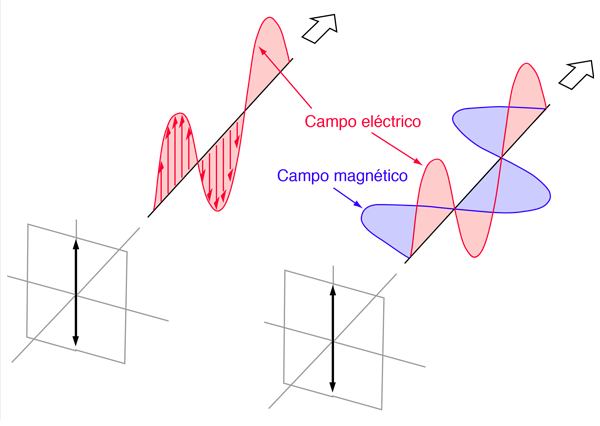
\includegraphics[width=0.5\linewidth]{Ant/Ant2.png}
\label{fig:pol lin}}
\subfloat[El vector de polarización gira 360º a medida de que la onda recorre una longitud de onda en el espacio]{
\includegraphics[width=0.5\linewidth]{Ant/Ant3.png}\label{fig:pol circ}}\\
\subfloat[Cuando la Intensidad de Campo varía con cambios en la polarización, se dice que es una Polarización Elíptica.]{
\includegraphics[width=0.5\linewidth]{Ant/Ant4.png}\label{fig:pol elip}}
\subfloat[Tipos de polarizaciones.]{
\includegraphics[width=0.5\linewidth]{Ant/Ant5.png}}
\caption{Polarización de ondas.}
\end{figure}
\begin{notation}
Si el vector gira en sentido de las manecillas del reloj, se dice que es Derecho, si es contrario se dice que es Izquierdo
\end{notation}
\subsubsection{Densidad de potencia radiada}
La \textbf{rapidez} con que la energía pasa a través de una \textbf{superficie} dada en el espacio libre se llama D\textbf{ensidad de Potencia}. La \textbf{Densidad de Potencia Radiada} se define como la potencia por unidad de superficie en una determinada dirección. Las unidades son \textbf{Watt por Metro Cuadrado} ($W/m^2$). Se puede calcular a partir de los valores eficaces de los campos eléctrico o magnéticos.
\begin{definition}[Potencia Isotrópica Radiada Equivalente]
\begin{equation}
PIRE=P_r\cdot D=P_A\cdot G
\label{eq:pire}
\end{equation}
Donde:
\begin{itemize}
\item PIRE:  Potencia Isotrópica Radiada Equivalente. (W)
\item $P_R$: Potencia de radiación.
\item $P_A$: Potencia suministrada a la antena. (W)
\item \textbf{G}: Ganancia.
\item \textbf{D}: Directividad de la antena.\footnote{Estos conceptos se detallan más adelante.}
\end{itemize}
\end{definition}
\begin{definition}[Intensidad de campo]
Es la intensidad de los campos eléctrico y magnético de una onda electromagnética que se propaga por el espacio libre.
\begin{equation}
\mathbb{P}=E\cdot H=\frac{PIRE}{4\pi r^2}=Z_s\times H^2=\frac{E^2}{Z_s}
\label{eq:int campo}
\end{equation}
Donde:
\begin{itemize}
\item $\mathbb{P}$: Densidad de potencia. ($W/m^2$)
\item \textbf{E}: Intensidad de campo eléctrico. (V/m)
\item \textbf{H}: Intensidad del campo magnético. (A/m)
\item \textbf{r}: Radio de la esfera. (m)
\item \textbf{\textit{PIRE}}: Potencia Isotrópica Radiada Equivalente. (W)
\end{itemize}
\end{definition}
\begin{definition}[Impedancia en el espacio libre]
La relación entre el módulo del campo eléctrico y el módulo del campo magnético es la impedancia característica del medio. La impedancia característica de un medio de transmisión \textbf{sin pérdidas} en igual a la raíz cuadrada de la relación de su permeabilidad magnética entre su permitividad eléctrica:
\begin{equation}
Z_s=\sqrt{\frac{\mu_0}{\epsilon_0}}=377\Omega
\label{eq:imp carac espacio libre}
\end{equation}
Donde:
\begin{itemize}
\item $Z_s$: Impedancia en el espacio libre. ($\Omega$)
\item $\mu_0$: Permeabilidad magnética ($1.26\basedec{-6}$H/m ó $4\pi\cdot K N/A^2$ donde $K=\basedec{-7}$).
\item $\epsilon_0$: Permitividad eléctrica del vacío ($8.85\basedec{-12}$F/m).
\end{itemize}
\end{definition}
%\begin{definition}[Potencia total radiada]
%Se puede obtener como la integral de la Densidad de Potencia en una esfera que encierre a la antena.
%\begin{equation}
%P_{tr}=\frac{P_{rad}}{4\pi r^2}
%\end{equation}
%\end{definition}
La \textbf{Intensidad de Radiación} es la potencia radiada por unidad de ángulo sólido en una determinada dirección.
\subsubsection{Ley de cuadrado inverso}
La \textbf{densidad de potencia} es inversamente proporcional al cuadrado de la distancia de la fuente.
\begin{equation}
\frac{\mathbb{P}_2}{\mathbb{P}_1}=\left(\frac{r_1}{r_2}\right)^2
\label{eq:ley cuadrado inverso}
\end{equation}
Para que se cumpla esta ley, la velocidad de propagación en todas las direcciones debe ser uniforme (Medio Isotrópico)
\subsubsection*{Atenuación y absorción}
\textbf{Atenuación} es la reducción de la Densidad de Potencia con la distancia. La atenuación se debe al esparcimiento esférico de la onda, se le llama ``atenuación espacial'' de la onda. Se expresa generalmente en términos del logaritmo de la relación de  densidad de  potencia (pérdida en dB)\\
\textbf{Absorción} solo se presenta cuando los CEM se propagan por la atmósfera. Es la energía transferida de la OEM a los átomos y las moléculas de la atmósfera. La absorción de radiofrecuencias en una atmósfera normal, es relativamente insignificante a frecuencias por debajo de 10 GHz.
\section{Antenas}
Las dos funciones primordiales de la antena son:
\begin{enumerate}
\item Convertir la energía electromagnética, procedente del generados a través de la línea de transmisión, en energía electromagnética que se propaga libremente por el espacio.
\item Adapta la impedancia interna del generador a la impedancia del espacio.
\end{enumerate}
En las líneas de transmisión se propagan ondas electromagnéticas \textbf{guiadas}, es decir campos electromagnéticos variables entre cargas y corrientes. Las antenas convierten estos ondas electromagnéticas guiadas en \textbf{libres} y \textbf{viceversa}. Tanto las ondas guiada como las libres son señales de radio.\\
En el proceso de su propagación, las ondas de radio se \textbf{dispersan} más allá de las líneas de radio-comunicación y son absorbidas por el medio circundante. Si la dirección de radiocomunicación es conocida y limitada, las perdidas pueden reducirse concentrando las ondas emitidas en direcciones definidas.
\subsection{Tipos de antenas}
A grandes rasgos existen dos tipos de antenas: antenas de \textbf{transmisión} y antenas de \textbf{recepción}.
\subsubsection*{Antenas de transmisión}
La antena de transmisión transforma energía de un campo electromagnético estacionario producido por la señal de radio, en energía de un campo electromagnético de radiación, añadiendo además que este último debe emitirse en unas direcciones dadas.
\subsubsection*{Antenas de recepción}
La antena de recepción está destinada a la transformación de la energía de una radioseñal consistente en un campo de radiación que procede de una dirección dada, en energía de un campo estacionario de ondas electromagnéticas.
\begin{remark}
La antena de transmisión y recepción tienen procesos \textbf{recíprocos}. Esto quiere decir que existe la posibilidad de utilizar la misma antena en calidad de transmisora y de receptora, y de conservar invariables los parámetros principales de la antena.
\end{remark}
\subsection{Características y parámetros de las antenas transmisoras}
\begin{definition}[Potencia de radiación y resistencia de radiación]
Representa la característica de la antena para la emisión energía electromagnética.
\begin{equation}
R_r=\frac{P_r}{i^2}
\label{eq:resistencia radiacion}
\end{equation}
Donde:
\begin{itemize}
\item $R_r$: Resistencia de radiación. ($\Omega$)
\item $P_r$: Potencia de radiación. (W)
\item \textbf{i}: Valor eficaz de la corriente de la antena. (A)
\end{itemize}
\end{definition}
Cuantitativamente la resistencia de radiación de define como aquella resistencia pura en la que se libera una potencia numéricamente igual a la potencia de radiación, para una corriente en la resistencia igual ala corriente en la antena.
\begin{definition}[Potencia de Pérdidas y resistencia de pérdidas]
Potencia que se pierde por el calentamiento del conductor, en los aisladores, en la tierra y en los objetos situados cerca de la antena.
\begin{equation*}
R_p=\frac{P_p}{i^2}
\label{eq:resistencia perdidas}
\end{equation*}
Donde:
\begin{itemize}
\item $R_p$: Resistencia de pérdidas. ($\Omega$)
\item $P_p$: Potencia de pérdidas. (W)
\item \textbf{i}: Valor eficaz de la corriente de la antena.
\end{itemize}
\end{definition}
\begin{definition}[Potencia de una antena y resistencia activa total o resistencia de antena]
Resistencia que corresponde a potencia suministrada a la antena. Potencia de antena es la suministrada a la antena por el transmisor, a través de la línea de transmisión, se obtiene con la suma de la potencia de \textbf{radiación} y la potencia de \textbf{pérdidas}.
\begin{equation}
P_A=P_r+P_p=i^2\left(R_r+R_p\right)
\label{eq:potencia antena}
\end{equation}
\begin{equation}
R_A=R_r+R_p
\end{equation}
Donde:
\begin{itemize}
\item $P_A$: Potencia suministrada a la antena. (W)
\item $P_r$: Potencia de radiación. (W)
\item $P_p$: Potencia de pérdidas. (W)
\item \textbf{i}: Valor eficaz de la corriente de la antena. (A)
\item $R_r$: Resistencia de radiación. ($\Omega$)
\item $R_p$: Resistencia de pérdidas. ($\Omega$)
\item $R_A$: Resistencia activa total. ($\Omega$)
\end{itemize}
\end{definition}
\begin{definition}[Rendimiento o Eficacia de una antena]
Es la relación entre la Potencia de Radiación y la Potencia Suministrada a la Antena.
\begin{equation*}
\eta_A=\frac{P_r}{P_A}=\frac{R_r}{R_r+R_p}=\frac{R_r}{R_A}=\frac{G}{D}
\label{eq:rendimiento de antena}
\end{equation*}
\begin{displaymath}
0\leq\eta_A\leq 1
\end{displaymath}
Donde:
\begin{itemize}
\item $\eta_A$: Rendimiento de antena.
\item $P_A$: Potencia suministrada a la antena. (W)
\item $P_r$: Potencia de radiación. (W)
\item $R_r$: Resistencia de radiación. ($\Omega$)
\item $R_p$: Resistencia de pérdidas. ($\Omega$)
\item $R_A$: Resistencia activa total. ($\Omega$)
\item \textbf{G}: Ganancia.
\item \textbf{D}: Directividad.
\end{itemize}
\end{definition}
\subsection{Parámetros de acción directiva de antenas}\index{Parámetros de acción directiva de antenas}
\subsubsection{Directividad}
La característica de directividad de antena muestra la \textbf{dependencia} de la intensidad de campo de radiación respecto a la dirección, con la condición que este campo sea medido siempre a igual distancia de la antena. Para el estudio de la radiación de una antena, se supone que la antena está situada en el punto medio de una ``esfera'' y en el origen de un sistema de coordenadas espaciales.
En la superficie de la ``esfera'' se calcula E y H en cualquier punto de esta, alejado una distancia \textit{r} del centro del dipolo.\\
\textbf{Características:}
\begin{enumerate}
\item \textbf{Propiedad Directiva}: Todas las antenas reales tienden a concentrar los campos radiado en alguna dirección.
\item \textbf{Característica de Directividad}: Depende de la intensidad de campo de radiación, respecto a la dirección, medido siempre a igual distancia de la antena. 
\item \textbf{Función de Directividad}: Expresión matemática de la directividad.
\begin{displaymath}
f^2(\theta,\phi)
\end{displaymath}
\item \textbf{Diagrama de Directividad}: Representación gráfica de la función de directividad. Normalmente se expresa en proyecciones:
\begin{enumerate}
\item Plano Horizontal ( $\phi$ varía y $\theta$ = 90º)
\item Plano Vertical ( $\theta$ varía y $\phi$	 = 0º)
\end{enumerate}
\end{enumerate}
\begin{definition}[Factor de directividad]
Factor de Directividad es la relación entre la densidad del flujo de potencia emitido por la antena dada en una \textbf{determinada dirección}, y la densidad de flujo de potencia que emitiría una antena absolutamente \textbf{no direccional} en cualquier dirección, siendo iguales las potencias totales de radiación de ambas antenas y medido a igual distancia.
\begin{equation}
D=\frac{\mathbb{P}_{max}}{\mathbb{P}_{ref}}=\frac{E_{max}^2}{E_0^2}
\label{eq:directividad}
\end{equation}
Donde:
\begin{itemize}
\item \textbf{D}: Factor de directividad.
\item $\mathbb{P}_{max}$: Densidad de potencia en un punto, en la dirección de máxima radiación. ($W/m^2$)
\item $\mathbb{P}_{ref}$: Densidad de potencia en el mismo punto, con una antena no direccional o de referencia. ($W/m^2$)
\end{itemize}
\end{definition}
\begin{definition}[Ganancia de potencia]
\begin{equation}
G=\eta_A\cdot D=\frac{\mathbb{P}_{max}}{\mathbb{P}_{ref}'}
\label{eq:ganancia}
\end{equation}
Donde:
\begin{itemize}
\item \textbf{G}: Ganancia.
\item $\eta_A$: Rendimiento de la antena.
\item \textbf{D}: Directividad de la antena.
\item $\mathbb{P}_{max}$: Densidad de potencia en un punto, en la dirección de máxima radiación. ($W/m^2$)
\item $\mathbb{P}_{ref}'$: Densidad de potencia en el mismo punto, con una antena no direccional o de referencia sin pérdidas. ($W/m^2$)
\end{itemize}
\end{definition}
\begin{definition}[Factor de calidad]
\begin{equation}
Q=\frac{f_r}{BW}
\label{eq:factor de calidad}
\end{equation}
Donde:
\begin{itemize}
\item Q: Factor de calidad.
\item $f_r$: Frecuencia de resonancia. (Hz)
\item $BW$: Ancho de banda. (Hz)
\end{itemize}
\end{definition}
\subsection{Antenas receptoras}
\begin{definition}[Área de captura]
Mientras que la \textbf{ganancia de potencia} es el parametro natural para describir la mayor densidad de potencia de una señal transmitida, por las propiedades direccionales de la antena transmisora, para describir las propiedades receptiras de una antena se usa una cantidad relacionada: \textbf{área de captura}
\begin{equation}
A_{cap}=\frac{G_r\cdot\lambda^2}{4\pi}
\label{eq:area capturada}
\end{equation}
Donde:
\begin{itemize}
\item $A_{cap}$: Área efectiva de captura. ($m^2$)
\item $G_r$: Ganancia del receptor.
\item $\lambda$: Longitud de onda de la señal recibida. (m)
\end{itemize}
\end{definition}
\begin{definition}[Potencia capturada]
Potencia disponible en las terminales de salida de la antena receptora. La potencia capturada es directamente proporcional a la densidad de potencia recibida y al área de captura de la antena receptora.
\begin{equation}
P_{cap}=\mathbb{P}\cdot A_{cap}
\label{eq:potencia capturada}
\end{equation}
Donde:
\begin{itemize}
\item $P_{cap}$: Potencia capturada. (W)
\item $\mathbb{P}$: Densidad de potencia capturada. ($W/m^2$)
\item $A_{cap}$: Área capturada. ($m^2$)
\end{itemize}
\end{definition}
%----------------------------------------------------------------------------------------
%	NEW CHAPTER
%----------------------------------------------------------------------------------------
\part{Internetworking 2}
\chapterimage{chapter_head_IT2.pdf} % Chapter heading image

\chapter{Unidad I}
\section{Protocolo spanning tree}\index{Protocolo spanning tree}
El algoritmo \textbf{Spanning Tree} (árbol de expansión) se utiliza en los switches para prevenir los bucles lógicos que pueden aparecer en una red. Los bucles se producen cuando existen varios caminos distintos entre dos puntos de la red y su efecto es que las tramas pueden circular de forma indefinida atrapadas en un bucle sin conseguir alcanzar su destino, lo que además afectará negativamente al rendimiento de la red. El algoritmo \textit{Spanning Tree} ayuda a los switches a elegir el camino más idóneo y, por tanto, elimina los bucles.
\begin{notation}
El protocolo \textit{spanning tree esta detallado especificado en el estándar \textbf{IEEE 802.1D}. Existe su variante con funcionamiento optimizado: \textbf{spanning tree rápido}-IEEE 802.1w}
\end{notation}

%----------------------------------------------------------------------------------------
%	NEW CHAPTER
%----------------------------------------------------------------------------------------
\part{Control Adaptativo Moderno}
\chapterimage{chapter_head_CAM.pdf} % Chapter heading image

\chapter{Unidad I}
%----------------------------------------------------------------------------------------
%	NEW CHAPTER
%----------------------------------------------------------------------------------------
\part{Software de telecomunicaciones}
\chapterimage{chapter_head_SFT.pdf} % Chapter heading image

\chapter{Unidad I}
%----------------------------------------------------------------------------------------
%	NEW CHAPTER
%----------------------------------------------------------------------------------------
\part{Microelectrónica en radiofrecuencia}
\chapterimage{chapter_head_MR.pdf} % Chapter heading image

\chapter{Unidad I}
%----------------------------------------------------------------------------------------
%	ANEXOS
%----------------------------------------------------------------------------------------
\part{Anexos}
%---------------------------------------------------------------
% 		ENDING
%---------------------------------------------------------------
\stopcontents[part] % Manually stop the 'part' table of contents here so the previous Part page table of contents doesn't list the following chapters

%----------------------------------------------------------------------------------------
%	BIBLIOGRAPHY
%----------------------------------------------------------------------------------------

\chapterimage{Final2.jpg} % Chapter heading image
\chapterspaceabove{6.75cm} % Whitespace from the top of the page to the chapter title on chapter pages
\chapterspacebelow{7.25cm} % Amount of vertical whitespace from the top margin to the start of the text on chapter pages

%------------------------------------------------
\chapter*{Bibliography}
\markboth{\sffamily\normalsize\bfseries Bibliography}{\sffamily\normalsize\bfseries Bibliography} % Set the page headers to display a Bibliography chapter name
\addcontentsline{toc}{chapter}{\textcolor{ocre}{Bibliography}} % Add a Bibliography heading to the table of contents

\section*{Articles}
\addcontentsline{toc}{section}{Articles} % Add the Articles subheading to the table of contents

%\printbibliography[heading=bibempty,type=article] % Output article bibliography entries

\section*{Books}
\addcontentsline{toc}{section}{Books} % Add the Books subheading to the table of contents

\printbibliography[heading=bibempty,type=book] % Output book bibliography entries
%----------------------------------------------------------------------------------------
%	APPENDICES
%----------------------------------------------------------------------------------------
%
%\chapterimage{Final1.jpg} % Chapter heading image
%\chapterspaceabove{6.75cm} % Whitespace from the top of the page to the chapter title on chapter pages
%\chapterspacebelow{7.25cm} % Amount of vertical whitespace from the top margin to the start of the text on chapter pages
%
%\begin{appendices}
%
%\renewcommand{\chaptername}{Appendix} % Change the chapter name to Appendix, i.e. "Appendix A: Title", instead of "Chapter A: Title" in the headers
%
%%------------------------------------------------
%
%\chapter{Appendix Chapter Title}
%
%\section{Appendix Section Title}
%
%Lorem ipsum dolor sit amet, consectetur adipiscing elit. Aliquam auctor mi risus, quis tempor libero hendrerit at. Duis hendrerit placerat quam et semper. Nam ultricies metus vehicula arcu viverra, vel ullamcorper justo elementum. Pellentesque vel mi ac lectus cursus posuere et nec ex. Fusce quis mauris egestas lacus commodo venenatis. Ut at arcu lectus. Donec et urna nunc. Morbi eu nisl cursus sapien eleifend tincidunt quis quis est. Donec ut orci ex. Praesent ligula enim, ullamcorper non lorem a, ultrices volutpat dolor. Nullam at imperdiet urna. Pellentesque nec velit eget est euismod pretium.
%
%%------------------------------------------------
%
%\chapter{Appendix Chapter Title}
%
%\section{Appendix Section Title}
%
%Lorem ipsum dolor sit amet, consectetur adipiscing elit. Aliquam auctor mi risus, quis tempor libero hendrerit at. Duis hendrerit placerat quam et semper. Nam ultricies metus vehicula arcu viverra, vel ullamcorper justo elementum. Pellentesque vel mi ac lectus cursus posuere et nec ex. Fusce quis mauris egestas lacus commodo venenatis. Ut at arcu lectus. Donec et urna nunc. Morbi eu nisl cursus sapien eleifend tincidunt quis quis est. Donec ut orci ex. Praesent ligula enim, ullamcorper non lorem a, ultrices volutpat dolor. Nullam at imperdiet urna. Pellentesque nec velit eget est euismod pretium.
%
%%------------------------------------------------
%
%\end{appendices}
%----------------------------------------------------------------------------------------
%	INDEX
%----------------------------------------------------------------------------------------

\cleardoublepage % Make sure the index starts on an odd (right side) page
\phantomsection
\setlength{\columnsep}{0.75cm} % Space between the 2 columns of the index
\addcontentsline{toc}{chapter}{\textcolor{ocre}{Index}} % Add an Index heading to the table of contents
\printindex % Output the index
%----------------------------------------------------------------------------------------
%	CHAPTER
%----------------------------------------------------------------------------------------

\end{document}
